\documentclass[12pt]{article}
\usepackage{geometry}
\usepackage{amsmath}
\usepackage{amssymb}
\usepackage{enumitem}
\usepackage{fancyhdr}
\usepackage{tikz}
\usepackage{color}
\usepackage{xspace}
\usepackage{thumbpdf}
\usepackage{listings}
\usepackage{verbatim}
\usepackage{hyperref}
\usepackage{booktabs}
\usepackage{colortbl}
\usetikzlibrary{trees}
\pagestyle{fancy}

\newcommand{\xref}[1]{\S\ref{#1}}
\definecolor{darkred}{rgb}{0.7,0,0}
\definecolor{darkgreen}{rgb}{0,0.5,0}
\hypersetup{colorlinks=true,
	linkcolor=darkred,
	citecolor=darkgreen}

\lstset{
	basicstyle=\ttfamily,
	mathescape
}

\lstdefinestyle{customc}{
	belowcaptionskip=1\baselineskip,
	breaklines=true,
	% xleftmargin=20pt,
	language=matlab,
	% frame=L,
	escapeinside={@}{@},
	showstringspaces=false,
	basicstyle=\small\ttfamily,
	keywordstyle=\bfseries\color{green!40!black},
	commentstyle=\itshape\color{purple!40!black},
	%identifierstyle=\color{blue},
	stringstyle=\color{orange},
	% directivestyle=\color{brown},
	%numbers=left,
	%numberstyle=\tiny\color{gray}
}

\lstdefinestyle{customctable}{
	aboveskip=-\medskipamount,
	belowskip=-\medskipamount,
	language=C,
	escapeinside={@}{@},
	showstringspaces=false,
	basicstyle=\scriptsize\ttfamily,
	keywordstyle=\bfseries\color{green!40!black},
	commentstyle=\itshape\color{purple!40!black},
	%identifierstyle=\color{blue},
	stringstyle=\color{orange},
	directivestyle=\color{brown},
}

\textheight=8.5in

\lhead{6.854 Pset 2}
\chead{Hongzi Mao}
\rhead{Spet 21, 2016}

\begin{document}
	
\section*{Problem 1}
\paragraph{(a)}
\subparagraph{Algorithm}
~\\

In \textbf{Init}, together with the original n-element array \textbf{arr}, we initialize two other arrays, called \textbf{from} and \textbf{to} (leave their entries untouched). In addition, a single integer \textbf{num} is initialized to 0. 

\textbf{Set}(i, x) first invokes \textbf{Get}(i). If the result not ``empty'', it sets \textbf{arr}[i] $:= x$. Otherwise, it sets the following
\begin{itemize}
	\item \textbf{from}[i] $:=$ \textbf{num}
	\item \textbf{to}[\textbf{num}] $:=$ i
	\item \textbf{num} $:=$ \textbf{num} + 1
	\item \textbf{arr}[i] $:= x$
\end{itemize}

\textbf{Get}(i) checks if \emph{both} \textbf{from}[i] $<$ \textbf{num} \emph{and} \textbf{to}[\textbf{from}$[i]$] $==$ i, then returns \textbf{arr}[i], otherwise returns ``empty''.
\subparagraph{Analysis}
~\\

The integer \textbf{num} indicates total number of entries that the original array is being used. \textbf{from} redirects the query entry to \textbf{to}, which stores the `actual' entry being set in the first time. Notice that the element in \textbf{to} array indexing from 1 to \textbf{num} is correct and uniquely pointing to entries in \textbf{arr}, which in and only in the correct case, will map back the query $i$, namely \textbf{to}[\textbf{from}[$i$]] $= i$. This will not be disturbed by any garbage in the system.

Initializing the original \textbf{arr}, \textbf{from}, \textbf{to} and \textbf{num}, takes $O(1)$ each, therefore $O(1)$ in total. 

\textbf{Get} and \textbf{Set} only uses constant number array lookup and arithmetic comparison, and thus is $O(1)$ as well. 

\pagebreak

\section*{Problem 2}

To implement Dijkstra's algorithm, we need to store the minimum known distance in the graph that is not being marked 'checked'. In the vanilla way of implementing it, we do need to use $O(log\:log\: nC)$ space, for all possible distances. 

However, notice that the distance of any node to any other node is bounded by $C$ (Triangle Inequality). This means that we can construct a `ring' structure to capture the distance of all other nodes starting from the current shortest distance node. 

Specifically, we construct \emph{two} vEB priority queue. When computing the distance $d$ to a node, we store $d \: mod \: C$ (key for queue) along with $\lfloor d/C\rfloor$ (extra field). Denote the distance of current fingering node as $d^*$, for the distances to other nodes, if the newly computed shortest distance $d$ satisfying $d \: mod \: C > d^* \: mod \: C$, we put $d \: mod \: C$ in the \emph{second} vEB priority queue; otherwise, we put it in the \emph{first} vEB queue. 

Now in order to iterate to the next node, we look into the \emph{second} vEB queue and invoke \emph{find-min}, if the return is invalid (meaning the second vEB queue is empty), we invoke \emph{find-min} in the first vEB queue. The real distance can be retrieved by using both $d \: mod \: C$ along with $\lfloor d/C\rfloor$ being stored.

The reason this two vEB queue works is that they effectively construct a `ring' structure. The starting point (distance to the current node) sits in the middle to first queue. Then, the next known minimum distance to all other nodes is immediately after the current distance after taking $mod\:C$ operation and will be put in the second queue. If it rotates back, it will be the first element in the first queue. Because the next minimum distance is bounded to be at most $C$ greater than current distance, two queues each with size $C$ is enough.

Therefore, we actually only need $O(log\:log\:C)$ for vEB queue operation in Dijkstra's algorithm.

\emph{\big(In a hindsight, we can achieve similar conclusions with one vEB tree from ideas in problem 3. Same $(d\:mod\:C)$ trick but The next-find-min operation can be replaced by successor, and the rotation happens when successor hits an invalid answer and we invoke getting minimum in tree.\big)}

\pagebreak

\section*{Problem 3}
To construct a data structure to support queries for existence of element, its predecessor and successor, we maintain an `array' with entry 1 indicating existence of element and 0 otherwise. We build vEB version of it to reach $O(log\:log\:u)$ operation time. 

For integer $x$ in range $\{0, 1, 2, ..., u-1\}$, define $x.high = \lfloor \frac{x}{\sqrt{u}} \rfloor$, and $x.low = x\:\text{mod}\:\sqrt{u}$. Note $x = x.high \times \sqrt{u} + x.low$. Split $Q$ into $\sqrt{u}$ clusters, each having $\sqrt{u}$ entries. Construct an array with size $\sqrt{u}$ whose entries store the \textbf{summary} (if there is at least one element, 1 indicating existence, 0 otherwise) in each cluster.

\subparagraph{Find(x, Q)} 
~\\

(1). Check if $Q.summary(x.high)$ is 1.

(2). If (1) holds, check if $Q.cluster[x.high][x.low]$ is 1.

Report existence if both (1) and (2) holds, non-existence otherwise.

\subparagraph{Predecessor(x, Q)} 
~\\

\emph{(If $Q$ is in the top or bottom level, namely no Q.summary or Q.cluster, it finds predecessor in the current level and abort with $-\infty$ if operation invalid.)}

$i := x.high$

$j:=$ the largest index with value 1, that is smaller than $x.low$. 

If $j$ is not valid: 

$\:\:\:\:i:= $ \textbf{Predecessor}($x.high, Q.summary$)

$\:\:\:\:j:= $ \textbf{Predecessor}($+\infty, Q.cluster[i]$)

return $i \times \sqrt{u} + j$.

\subparagraph{Successor(x, Q)} 
~\\

\emph{(If $Q$ is in the top or bottom level, namely no Q.summary or Q.cluster, it finds successor in the current level and abort with $+\infty$ if operation invalid.)}

$i := x.high$

$j:=$ the smallest index with value 1, that is larger than $x.low$. 

If $j$ is not valid: 

$\:\:\:\:i:= $ \textbf{Successor}($x.high, Q.summary$)

$\:\:\:\:j:= $ \textbf{Successor}($-\infty, Q.cluster[i]$)

return $i \times \sqrt{u} + j$.
~\\

\subparagraph{Analysis} 
~\\

Notice that the number of levels of \emph{summary-cluster} is $O(log\:log\:n)$. This is because of the following. Notice that every one level up, the summary aggregates $\sqrt{n}$ nodes. To get the number of levels, we essentially need to get `` how many $1/2$ are there in $((u^{1/2})^{1/2})^{...}$ to reach 1. Let $v = log(u)$, then it becomes $e^{\frac{1}{2}\frac{1}{2}...v}$ and we know here the number of $1/2$ will be $log\:v = log\:log\:u$.

In the \textbf{find} step, the level of tree determines the worst-case query time, which is $O(log\:log\:u)$.

In \textbf{predecessor} and \textbf{successor} step, we use recursion analysis to calculate the run time $T(u)$. Because every time it breaks the cluster into size $\sqrt{u}$ and searching in the $summary$ and $cluster$ both takes $O(\sqrt{u})$, we will have 
$$ T(u) = T(\sqrt{u}) + O(1).$$ Now we replace $v = log(u)$, then $ T(v) = T(\frac{1}{2}v) + O(1)$, and we get $T(v) = O(log(v))$, therefore $T(u) = O(log(T(v))) = O(log\:log\:u)$. (This is similar to the analysis for \textbf{find}).

~\\

\textbf{Find-min} can be implemented by invoking \textbf{Successor}$(-\infty, Q)$, which has worst-case $O(log\:log\:n)$ time. \textbf{Delete-min} can use \textbf{find-min} first, then invoking \textbf{Successor}(\textbf{Find-min}(x, Q), Q), but along the path of going to the summary, appropriately marking the value to be 0, if the value in the cluster is deleted and the successor is not in the current cluster (In the above \textbf{Successor} algorithm, when $j$ is not valid, mark the summary to be $0$ as well.). This extra marking takes $O(1)$ time, therefore the worst-case time is still $O(log\:log\:n)$.

\pagebreak

\section*{Problem 4}
\paragraph{(a)}
First compute the probability for $k^{th}$ insertion being a collision. A collision happens when there are at least one item in the same entry in \emph{both} arrays. This means previously at least two items need to be mapped to this entry, which has probability $$p_k = 1 - \left(\frac{n^{1.5} - 1}{n^{1.5}}\right)^{k-1} - (k-1) \frac{1}{n^{1.5}}\left(\frac{n^{1.5}-1}{n^{1.5}}\right)^{k-2}.$$

The expected number of collision can be calculated as follows, 
\begin{align*}
\sum_{k=2}^n p_k &= \sum_{k=2}^n \left[1 - \left(\frac{n^{1.5} - 1}{n^{1.5}}\right)^{k-1} - (k-1) \frac{1}{n^{1.5}}\left(\frac{n^{1.5}-1}{n^{1.5}}\right)^{k-2}\right]\\
&= n - \sum_{k=2}^{n} \left(\frac{n^{1.5} - 1}{n^{1.5}}\right)^{k-1} - \sum_{k=2}^{n}(k-1) \frac{1}{n^{1.5}}\left(\frac{n^{1.5}-1}{n^{1.5}}\right)^{k-2}\\
&\leq n - \sum_{k=2}^{n}\left( 1 - \alpha\frac{k-1}{n^{1.5}}\right) - \sum_{k=2}^{n}(k-1)\frac{1}{n^{1.5}}\left(1-\alpha\frac{k-2}{n^{1.5}}\right)\\
&(\text{from Taylor expasion, where } \alpha = 1 + \epsilon \text{ to make ``$\leq$'' hold})\\
& = \frac{1}{3} (2n - 3n^2 + n^3) \frac{\alpha}{n^3}\\
&\leq \frac{\alpha}{3} = O(1)
\end{align*}

Notice that this computes the expected number of occurrence of \emph{any} item, which is bounded by $O(1)$. Then the (strange ``i.e.'' in the problem) expected number of pairs of item in the same bucket is also $O(1)$ (otherwise the number of collisions happened more often that $O(1)$).

\emph{Alternatively, we can use method in part (b) to prove the results here.}
\paragraph{(b)}

%\emph{(In order to make the math work for the same conclusion with only pairwise independence, we relax the array space to be $O(n^{1.5})$, which is to some extend still similar to (a). We now need to allocate two arrays with size $(1+\delta) n^{1.5}$})

Now we need to show the above argument works even when only assuming pair-wise independence, such that we can apply 2-universal hashing family to achieve efficiency. 

For any item $i$, the probability that another item $j$ maps to same index as it, by pairwise independence, is $p_{ij} = \frac{1}{n^{1.5}}$. Therefore, the probability for $i$ to collide with any item, bounded by Boole's inequality 

$$ \cup_j\: p_{ij} \leq \sum_j p_{ij} = n \frac{1}{ n^{1.5}} = \frac{1}{ \sqrt{n}}$$

Notice that in bashing, a `real' collision happens when at least two items are colliding. Therefore the probability for collision is $(\frac{1}{ \sqrt{n}})^2 = \frac{1}{n}$. Also notice that this probability is computed for any item $i$, therefore the total expected number of collision is $n \frac{1}{n} = O(1)$. Same conclusion from (a) holds.

Now we can create a 2-universal hashing family and randomly select a hashing function from it for each hashing operation. Because 2-universal hashing is efficient, we know bashing can be implemented efficiently.

\paragraph{(c)} Because the expected number of collision is bounded by 1 (from (b) Boole's inequality). We know the probability of a hash family being perfect is a constant $p$, regardless of the size of $n$. In order to find the perfect hashing, one needs to try out hash families drawn from the 2-universal hashing universe. Then, throughout the probing, the probability of the hash family being \emph{not} perfect is expoentially decayed as $(1-p)^k$, $k$ is the trial number until finding perfect hashing. Therefore, as each probing takes $O(n)$, finding perfect hashing takes $O(n)$.

\paragraph{(d)} 

Similar to part (a), because there is a $3rd$ or $4th$ polynomial term in the $p_k$ computation, we need to make $n^{1.5} = n^{1 + 1/2}$ in bashing case, to be $n^{1 + 1/3}$ for trashing and $n^{1 + 1/4}$ for quashing. \emph{To reach conclusion in (b) and (c), we may need 3-universal and 4-universal hashing family.}

\pagebreak

\section*{Problem 5}
\paragraph{(a)}
For $s$ items in the table with probability $1/2$ of perfect placement, we know the expected number of trials to find a perfect hashing is 2, from Markov Inequality. This is computed by the following 
\begin{align*}
\mathbb{E} (\text{number of trials}) &= 1 \times \frac{1}{2} + 2 \times (\frac{1}{2})^2 + 3 \times (\frac{1}{2})^3 + ... + n\times(\frac{1}{2})^n + ... \\
& = \sum_{n=1}^{\infty}\left[n\times\frac{1}{2^n}\right]\\
& = 2
\end{align*} 
Now for $s$ items, we mark some break points as $\{1, 2, 4, 8, 16, ..., s\}$. Suppose at each break point, we do a rebuild, then the success probability in the next break point will be $1/2$ and the expected number of rebuild is $s$ for the next marking point. 

Because we are computing the upper bound, we now artificially introduce a rebuild at each rebuild. This bounds the result in the following sense. If it does not require a rebuild but we enforce one, the `real' rebuild will have a wider range of support than our enforced one (because it happens later). Therefore it suffices to compute the expected rebuild complexity for these marking point, as follows

\begin{align*}
\mathbb{E} (\text{cost of rebuild}) &\leq \mathbb{E} (\text{number of rebuild counting until each break point}) \\
& \times \mathbb{E}(\text{rebuild cost for items until break point}) \\
& = 2 \times \big(1 + 2 + 4 + 8 + 16 + ... + s\big)\\
& \leq 2 \times 3s \\
& = O(s) 
\end{align*} 

\paragraph{(b)}
From the scheme of constructing 2-level perfect hashing, we know $\mathbb{E}\left[\sum s_i^2\right] = O(n)$, this is because 
\begin{align*}
\mathbb{E}\left[\sum s_k^2\right] & = O\left[\sum_k \sum_{\text{number of pairs of } i, j \text{ collides in k}} 1\right] \:\:\:  (\text{Notice number of pairs of collision} \sim s_k^2)\\
& = O\left[\sum_{i,j} \text{(i, j in the same bucket)}\right]\\
& = O\left[\sum_{i,j}C_{ij}\right] \:\:\:\:\:\:\:  (C_{ij} = \text{Probability that i j collides})\\
&= O(n^2\times\frac{1}{n}) \:\:\:\:\:\: \text{(Note that top level has $n$ buckets)})\\ 
& = O(n).\text{(Note that top level has $n$ buckets)})
\end{align*}

From Markov Inequality we know\footnote{We can set $\mathbb{E}\left[\sum s_k^2\right] = \alpha n$, and use $2\alpha n$ in Markov Inequality analysis to be more rigorous.} the $Pr(\sum s_i^2 > 2 \times O(n) = O(n)) < \frac{1}{2}$. Thus the expected number of attempts before getting a desired hashing is 2 (same argument from (a)).

Now in the similar argument as in (a), on the top level, the overall cost of rebuild is the same as (a), $O(n)$, because of the same expected attempt. 

For the second level, in each bucket, we need to consider the rebuild cost for (1) top level rebuilds and (2) collision happened in second level hashing. For case (1), we know the expected number of trials in each bucket is 2, and by the same argument, the rebuild cost is $O(k)$ where $k$ is the current inserted number of items. For case (2), every time a violation happens, it takes $O(b_k)$ to rebuild, where$b_k$ is number of items in bucket $k$. 

Using the same technique in (a), 

\begin{align*}
\mathbb{E} (\text{cost of rebuild}) &\leq \mathbb{E} (\text{top level rebuilds until each break point}) \\
& \times \mathbb{E}(\text{rebuild cost for all items until break point in both levels}) \\
&+ \mathbb{E} (\text{second level rebuilds until each break point}) \\
& \times \mathbb{E}(\text{rebuild cost for \emph{all} items in each bucket}) \\
& = 2 \times \big(1 + 2 + 4 + 8 + 16 + ... + s\big)\\
& + 2 \times \big(1 + 2 + 4 + 8 + 16 + ... + s\big) \:\:\:\: (\text{sum of all items in buckets will be $k$})\\
& \leq 4 \times 3s \\
& = O(s) 
\end{align*} 

\paragraph{(c)}
\emph{(The amortized cost $O(1)$ follows from the total cost $O(n)$ for $n$ insertion in (a). We follow the notions in (a) here.)} 

We need to keep another integer keeping track of number of valid items in the table. The delete clean up only happens when there are $n$ items in the table but only $n/2$ of it is valid. For number of items ranging between $n/2$ and $n$, we know the cost for all operations and analysis above only scaled by factor of 2, wouldn't affect $O(\cdot)$. In the extreme case, deleting items all the way down to 0 we need to at least rebuild when the valid item reduces to $n/2, n/4, n/8...$. Notice that in each rebuild, the cost is $O(k)$, where $k$ is the number of valid items in the system. Therefore the total cost is $O(n/2 + n/4 + n/8 + ...) = O(n)$ for such deletions, which can be charged against the inserts.

\pagebreak

\section*{Problem 6}
\paragraph{(a)}
\subparagraph{Algorithm} The pseudocode is as follows,
~\\

\begin{lstlisting}[style=customc]
	counter := $1$
	register := empty
	while streaming:
	  if register not empty and register == IP:
	      counter += 1
	  else:
	      counter -= 1
	  end if
	  
	  if counter == 0:
	      register := IP
	      counter := 1		
	  end if
	  
	end while
\end{lstlisting}

\subparagraph{Analysis}

Because we don't care about the IP in the register if it is not dominating at least half of all IPs, we only need to show that it captures the right IP when it appears at least half of the time.

We prove this by contradiction. Suppose another IP $j$ is the output other than the true dominating IP $i$. The above algorithm means, there is a period of time, that $j$ starts to kick in and dominating the counter, because all IPs other than $j$ can't diminish the counter increment due to $j$'s appearance. Moreover, the fact that $j$ can kick it, means $i$ is not dominating in the period from beginning to $j$ takes over, otherwise $i$ would stay in the register. It is not immediately obvious that $i$ is not dominating the first period, because initially it needs to do some work to take its position hold by others. We extend the period from $i$ starts taking the register mirroring to $i$ first comes in, then it is clear for the domination, as in Figure \ref{fig:6-1}. Because $i$ is not dominating from beginning to $j$ takes over and not dominating in $j$'s dynasty, it is not the dominating IP. Contradiction occurs. 
\begin{figure}
	\centering
	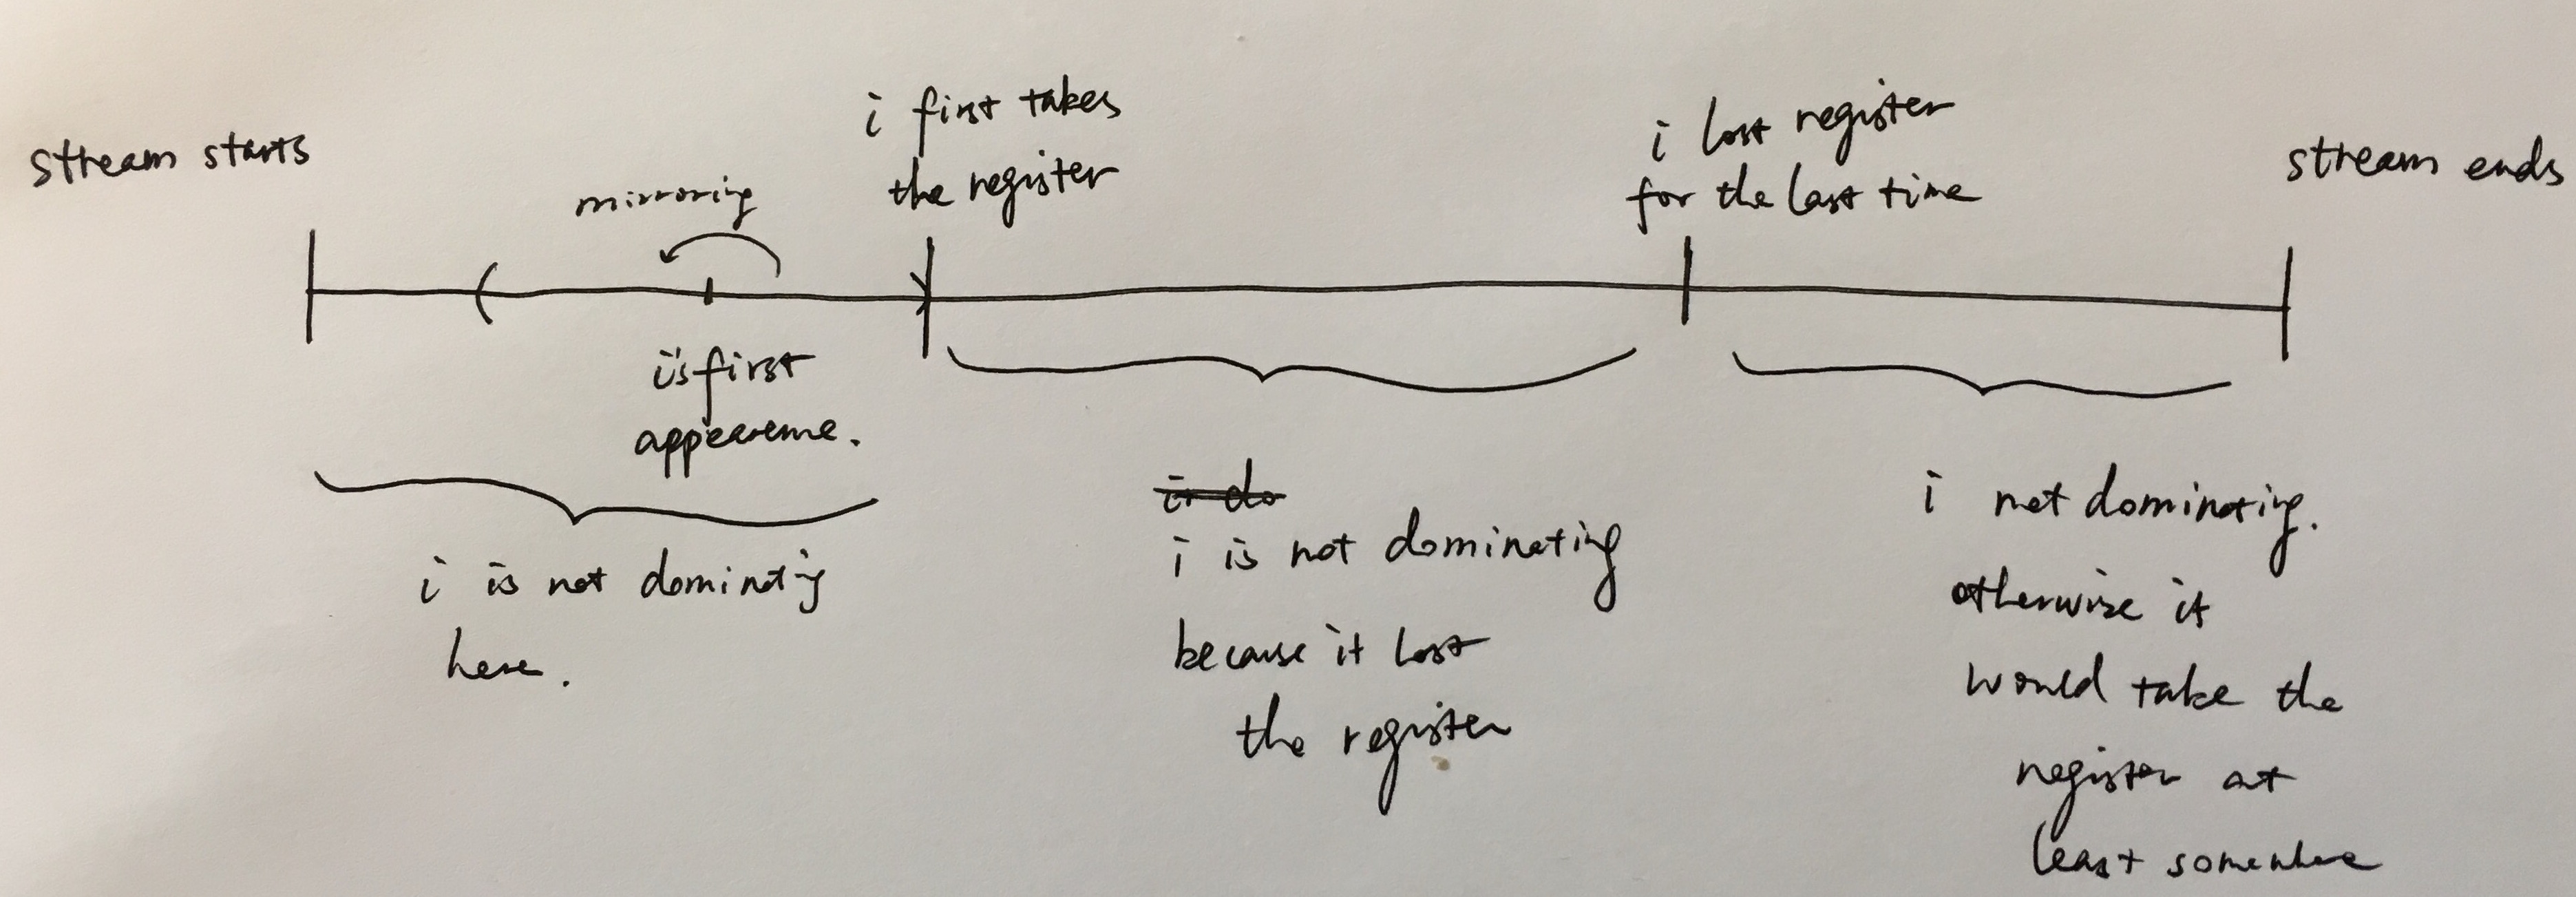
\includegraphics[width=0.7\textwidth]{6-1.jpg}
	\caption{Illustration of the stream.} \label{fig:6-1}
	\vspace*{-0.3in}
\end{figure}

\paragraph{(b)} \subparagraph{Algorithm} The extended pseudocode from (a) is as follows,

\begin{lstlisting}[style=customc]
	counter[1] := $1$, $i \in \{1, 2, 3, ..., k\}$
	register[$i$] := empty, $i \in \{1, 2, ..., k\}$
	
	while streaming:
	    stored := false
	    
	    for i in $\{1, 2, 3, ..., k\}$:
  	      if register[i] not empty and register[i] == IP:
	          counter[i] += k
	          stored := true
	      else:
	          counter[i] -= 1
	      end if
	    end for
	    
	    for i in $\{1, 2, 3, ..., k\}$:
	      if counter <= 0 and !stored:
	          register := IP
	          counter := k	
	          stored := true	
	      end if
	    end for
	end while
\end{lstlisting}

\subparagraph{Analysis} Very similar to part (a), we can use proof by contradiction to show the correctness of the algorithm. Suppose another IP $j$ is one of the outputs other than some other IP $i$ that contributes to $1/(k+1)$ of the traffic. The above algorithm means, there is a period of time, that $j$ starts to kick in and dominating one of the counter, because all IPs other than $j$ can't diminish the counter increment due to $j$'s appearance. Here the term `domination' means has at least $1/(k+1)$ of the traffic, because of the $+= k$ counting increment. Moreover, the fact that $j$ can kick it, means $i$ is not dominating in the period from beginning to $j$ takes over, otherwise $i$ would stay in the register. Because $i$ is not dominating from beginning to $j$ takes over and not dominating in $j$'s dynasty, it is not of $1/(k+1)$ of all IPs. Contradiction occurs. 

\end{document}